\documentclass[12pt]{article}
\usepackage{graphicx}
\usepackage{enumerate}
\usepackage{natbib}
\usepackage{url} % not crucial - just used below for the URL

%\pdfminorversion=4
% NOTE: To produce blinded version, replace "0" with "1" below.
\newcommand{\blind}{1}

% DON'T change margins - should be 1 inch all around.
\addtolength{\oddsidemargin}{-.5in}%
\addtolength{\evensidemargin}{-.5in}%
\addtolength{\textwidth}{1in}%
\addtolength{\textheight}{-.3in}%
\addtolength{\topmargin}{-.8in}%

\usepackage{amssymb}
\usepackage{amsmath}
\usepackage{theorem}
\usepackage{xfrac}
\usepackage{hyperref}

\DeclareMathOperator*{\argmin}{arg\,min}
\DeclareMathOperator*{\argmax}{arg\,max}
\newcommand{\sstar}{s^*}
\newcommand{\sfunc}{s}

\numberwithin{equation}{section}
\theoremstyle{plain}
\newtheorem{thm}{Theorem}[section]

\begin{document}

\def\spacingset#1{\renewcommand{\baselinestretch}%
{#1}\small\normalsize} \spacingset{1}


%%%%%%%%%%%%%%%%%%%%%%%%%%%%%%%%%%%%%%%%%%%%%%%%%%%%%%%%%%%%%%%%%%%%%%%%%%%%%%

\if1\blind
{
  \title{\bf Approximating Likelihood Ratios with Calibrated Discriminative Classifiers}
  \author{Kyle Cranmer and Gilles Louppe\\
          Center for Cosmology and Particle Physics, New York Univeristy}
  \maketitle
} \fi

\if0\blind
{
  \bigskip
  \bigskip
  \bigskip
  \begin{center}
    {\LARGE\bf Title}
\end{center}
  \medskip
} \fi

\bigskip
\begin{abstract}

In particle physics likelihood ratio tests are established tools for statistical
inference.  These tests are complicated by the fact that computer simulators are
used as a generative model for the data, but they do not provide a way to
evaluate the likelihood function. We demonstrate how discriminative classifiers
can be used to approximate the likelihood function when a generative model for
the data is available for training and calibration.  This offers an approach to
parametric inference when simulators are used that is complementary to
approximate Bayesian computation.

\end{abstract}

\noindent%
{\it Keywords:}  likelihood ratio, classification, particle physics
\vfill

\newpage
\spacingset{1.45} % DON'T change the spacing!

\section{Introduction}

The likelihood function is the central object that summarizes the information from an experiment needed for inference of model parameters. The likelihood function is key to Bayesian inference, and many areas of science that report the results of classical hypothesis tests or confidence intervals use the (generalized or profile) likelihood ratio as a test statistic.
It is increasingly common that a simulator (or generative model) is used to describe complex processes that tie
parameters $\theta$ of an underlying theory and measurement apparatus to high-dimensional observations $x$.
Directly evaluating the likelihood ratio in these cases is often impossible or is computationally impractical.
Approximate Bayesian Computation (ABC) is one approach to parameter inference in this simulation-based or likelihood-free setting~\citep{Rubin1984,Tavare1997,Marin2011}. Here we consider an alternative approach that can also be used in a classical setting where a prior over the parameters is not available. In particular, we demonstrate how discriminative classifiers can be used to construct equivalent likelihood ratio tests when a generative model for the data is available for training and calibration.

As a concrete example, consider searches for new particles at the Large Hadron Collider.
The simulator that is sampling from $p(x|\theta)$ is based on quantum field theory, a detailed simulation of the particle detector, and data processing algorithms that transform raw sensor data into the feature vector $x$~\citep{Sjostrand:2006za,Agostinelli:2002hh}.

The ATLAS and CMS experiments have published  hundreds papers where the
final  result was formulated as a hypothesis test or confidence interval
using a generalized  likelihood ratio test~\citep{Cowan:2010js}. This includes
the discovery of the Higgs boson~\citep{Aad:2012tfa,Chatrchyan:2012ufa} and
subsequent measurement of its properties.

The bulk of the likelihood ratio tests at the LHC are based on the distribution of a single event-level feature
that discriminates between a hypothesized process of interest (labeled \textit{signal}) and various other processes
(labeled \textit{background}). Typically,  pseudo-data from the simulator are used to approximate the density
at various parameter points, and an interpolation algorithm is used to approximate the parametrized model~\citep{Cranmer:2012sba}.

To improve the statistical power of these tests, hundreds of these searches have utilized supervised learning to train discriminative classifiers that take advantage of a high dimensional feature vector $x$. Within High Energy Physics (HEP) libraries such as TMVA that implement conventional techniques like the multi-layer perceptron and boosted decision trees~\citep{Hocker:2007ht} are commonly used. Recently, there has been progress in using deep networks~\citep{Baldi:2014kfa} and a NIPS workshop synthesizing the lessons learned during HiggsML~\citep{HepML}, the largest Kaggle challenge in history.

While classification accuracy can lead to optimal approaches for simple hypothesis tests~\citep{Dempster1965}, that is no longer true in the context of parameter estimation or composite hypothesis tests with nuisance parameters. As noted in ~\citep{Whiteson:2006ws}, ``such methods are suboptimal because they assume that the selector with the highest classification accuracy will yield a mass measurement with the smallest statistical uncertainty.''
The key distinction is that evaluating the loss for classification is composed of many per-event operations, while evaluating the loss for a mass measurement (e.g. the variance of an estimator for the mass parameter) is a per-experiment operation involving a data set with many events. They went on to demonstrate a computationally intensive stochastic optimization technique based on the per-experiment loss out performed the two stage selection-estimation process.

The initial motivation for this work was to extend the typical usage of discriminative classifiers in HEP to be robust to
nuisance parameters in the simulators. The scope of the result expanded once it became clear that this offers a way to approximate the likelihood function $p(x|\theta)$ in what is typically considered the likelihood-free setting. This approach is complementary to ABC as it does not require a prior over the parameters and can also be used in the classical (frequentist) setting. A strength of this approach is that it separates the quality of the approximation of the target likelihood from the quality of the calibration.  In Section~\ref{S:Related} we discuss the scheme sketched by \citep{Neal:2007zz} that also suggests using a classifier  as a dimensionality reduction map to aid in the estimation of the likelihood function.

\subsection{Notation and Assumptions}

We use the following notation:
\begin{itemize}
 \item $x$: a vector of features for an event
 \item $D$: a data set of $D=\{x_1, \dots, x_n\}$, where $x_e$ are assumed to be i.i.d.
 \item $\theta$: parameters of a statistical model
\item $p(x| \theta)$:  probability density  (simulation-based model) for $x$ given $\theta$
%\item $s(x)$: real-valued score from a machine learning classification algorithm (or any map $s: X\to\mathbb{R}$)
\item $y$: a class label used for training a classifier.
\item $s(x;\theta_0, \theta_1)$: real-valued discriminative classification score, parametrized by $\theta_0$ and $\theta_1$
%\item $p( s | \theta )$ The probability density function for $s$ implied by $p(x|\theta)$ and $s(x)$
\item $p( s_{\theta_0, \theta_1} | \theta )$: The probability density  for $s(x; \theta_0, \theta_1)$ implied by $p(x|\theta)$
\end{itemize}
We will assume the $x_e$ are i.i.d., so that $p(D|\theta) = \prod_{e=1}^n p(x_e | \theta)$.

%\newpage
\subsection{Prelude}

In the setting where one is interested in simple hypothesis testing between a null $\theta=\theta_0$ against an alternate $\theta=\theta_1$, the Neyman-Pearson lemma states that the likelihood ratio
\begin{equation}
T(D; \theta_0, \theta_1) = \prod_{e=1}^n \frac{ p(x_e|\theta_0)}{ p(x_e|\theta_1)}
\end{equation}
is the most powerful test statistic. In order to evaluate $T(D)$, one must be able to evaluate the probability density
$p(x| \theta)$ at any value $x$. However, it is increasingly common in science that one has a complex simulation that
can act as generative model  for $p(x|\theta)$, but one cannot evaluate the density directly. For instance, this is the case
high energy physics where the simulation of particle detectors can only be done in the `forward mode'. This same setting has been considered by \citep{ClaytonScott}, \citep{JMLR:v14:tong13a}, and \citep{Neal:2007zz}.

The main result of this paper is to generalize the observation that one can form an equivalent test based on
%\begin{equation}
%T'(D) = \prod_{e=1}^n \frac{ p(\,s(x_e; \theta_1, \theta_0) \mid \theta_1)}{ p(\,s(x_e; \theta_1, \theta_0)\mid\theta_0)}
%\end{equation}
\begin{equation}\label{eq:equivLRtest}
T'(D; \theta_0, \theta_1) = \prod_{e=1}^n \frac{ p(s_e | \theta_0)}{ p(s_e | \theta_1)}
\end{equation}
if
\begin{equation}\label{eq:montonic}
s_e = s(x_e; \theta_0, \theta_1) = m\left(\, p(x_e|\theta_0) / p(x_e|\theta_1) \,\right) \;
%s_e = s(x_e; \theta_0, \theta_1) = m\left(\frac{ p(x_e|\theta_0)}{ p(x_e|\theta_1)} \right) \;
\end{equation}
where $m$ is any strictly increasing or decreasing function. This result will be proven below.
This allows us to recast the original likelihood ratio test into an alternate form in which supervised learning is used to train the discriminative classifier $s(x; \theta_0, \theta_1)$. The discriminative classifier can be trained with data $(x,y=0)$ generated
from $p(x|\theta_0)$ and $(x,y=1)$ generated from $p(x|\theta_1)$. In Section~\ref{S:GLR} we extend this result to generalized likelihood ratio tests, where it will be useful to have the classifier  parametrized in terms of $(\theta_0, \theta_1)$.

Here we see that the original goal for simple hypothesis testing (i.e. to make a decision to accept or reject the null hypothesis based on the entire data set $D$) has been reformulated into a per-event classification problem. This follows from the fact that we assume the $x_e$ to be i.i.d.

\subsection{Comments on classification and frequentist hypothesis tests}

Vast literature exists around generative and discriminative classifiers~\citep{AndrewY.Ng}. Typically, generative classifiers learn a model for the joint probability $p(x,y)$, of the inputs $x$ and the classification label $y$, and predict $p(y|x)$ via Bayes rule. In contrast, discriminative classifiers model the posterior $p(y|x)$ directly. For classification tasks, one then thresholds on $p(y|x)$. In both cases this description in terms of a posterior requires a prior distribution for $p(y)$, which is either modeled explicitly or learned from the training data.
This familiar formulation of classification may lead to some confusion in the setting of the current work.

The first possible source of confusion we wish to avoid is that here $p(x|\theta)$  is a  \textit{generative statistical model} for the features $x$, not a generative classifier. We think of the  $p(x|\theta)$ along the lines of a traditional scientific theory or simulator, able to make predictions about $x$ and being motivated by domain-specific considerations.

The second possible source of confusion is that
we are not directly interested in calibrating the classification score in terms of a per-event posterior probability $p(y|x)$.
Instead, we are interested in the approximation of the per-experiment likelihood function or likelihood ratio, which might be used for several purposes, including the calculation of p-values.

Lastly, in the setting of frequentist hypothesis tests and confidence intervals, we do not have a prior $\pi(\theta)$.
While we can use the generative models to produce training data $(x,y=0)$ generated
from $p(x|\theta_0)$ and $(x,y=1)$ generated from $p(x|\theta_1)$, the relative mix $p(y)$
is arbitrary.  When $p(y=0)=p(y=1)=\sfrac{1}{2}$, then
\begin{equation}
p(y=1 | x) = \frac{p(x|y=1)}{p(x|y=0)+p(x|y=1)} = \frac{p(x|\theta_1)}{p(x|\theta_0)+p(x|\theta_1))} \;,
\end{equation}
which is monotonic with the desired likelihood ratio $p(x|\theta_1)/p(x|\theta_0)$.
Since the prior $p(y)$ is not needed for the target likelihood ratio test and because the classifier score $p(y|x)$ may not be well calibrated, we choose to denote the classifier score $s(x)$ and simply think of it as a deterministic dimensionality reduction map $s: X \to \mathbb{R}$.  Similar points have been made by~\citep{ClaytonScott} and \citep{Neal:2007zz}.



\section{Dimensionality reduction and calibration}


We are interested in reformulating the target likelihood ratio
\begin{equation}
\ln T(D; \theta_0, \theta_1) =   \sum_{e=1}^n \underbrace{\log \left[ \frac {p(x_e | \theta_0) }{ p(x_e | \theta_1) } \right]}_{q(x_e)} \;.
\end{equation}
Here we see that the test statistic $T$ for the experiment is composed of a sum over events of the per-event function $q(x)$. A sum over a monotonic, but non-linear function of $q(x)$ would not lead to an equivalent statistic.

The important part of the per-event function $q(x)$ is that it defines iso-contours in the feature space $x$. As we will show, our goal is to learn a monotonic function of $p(x|\theta_0)/p(x|\theta_1)$, which will share the same iso-contours. Then the remaining challenge is to find the appropriate monotonic function that gives back a linear function of $q(x)$. Our claim is that the generative model $p(x|\theta)$ can be used to calibrate the density $p(s|\theta)$ and that
\begin{equation}\label{eq:enveloping}
\ln T'(D; \theta_0, \theta_1) = \sum_{e=1}^n \underbrace{\log \left[ \frac {p(s_e | \theta_0) }{ p(s_e | \theta_1) } \right]}_{q(s_e)} \;,
\end{equation}
leads to an equivalent statistic.

For notational simplicity, let $p_0(x) = p(x|\theta_0)$, $p_1(x) = p(x|\theta_1)$, and $\sfunc(x)=s(x; \theta_0, \theta_1)$.
The distribution of $x$ totally determines the distribution of $s$.
In the application at hand, the function $s$ maps a high-dimensional feature vector $x$ to $\mathbb{R}^+$.
Let $\Omega_{\sstar}$ be the level set $\{x \mid s(x; \theta_0, \theta_1) = \sstar \}$ and \mbox{$\hat{n}=\nabla s(x) / |\nabla s(x)|$} be the orthonormal vector to $\Omega_{\sstar}$ at the point $x$.

We need to show that for all $x$, the density
\begin{equation}
p(q_x|\theta) = \int dx \delta(q_x-q_x(x)) p(x|\theta)  / | \hat{n} \cdot \nabla q_x  |
\end{equation}
is equal to the density
\begin{equation}
p(q_s|\theta) = \int dx \delta(q_s-q_s(s(x))) \, p(x|\theta) \, / | \hat{n} \cdot \nabla q_s  | \; .
\end{equation}
It is sufficient to show that $q_x(x) = q_s(s(x))$.
%$ \forall x\in\Omega_{\sstar}$.
The function $q_s(s)$ is based on the induced densities $p_0(s)$ and $p_1(s)$.  The induced density $p_1(s)$ is given by
\begin{equation}
p_1(\sstar) = \int dx \delta(\sstar-s(x)) p_1(x) = \int d\Omega_{\sstar} p_1(x)  / | \hat{n} \cdot \nabla s  |
\end{equation}
and a similar equation for $p_0(s)$.
%\textbf{Do we need Jacobian for x $\to$ s independent of delta function part, I think that's double counting?}

\textbf{\flushleft Theorem 1:}
We have the following equality
\begin{equation}
\frac{p_1(s(x))}{p_0(s(x))} =  \frac{p_1(x)}{p_0(x)}  \; . %\;\hspace{3em} \forall x\in\Omega_{\sstar}\; .
\end{equation}
\textbf{Proof}
For $x\in \Omega_{\sstar}$, we can factor out of the integral the constant $p_1(x)/p_0(x)$.
Thus
\begin{equation}
p_1(\sstar) =  \int d\Omega_{\sstar} p_1(x) / | \hat{n} \cdot \nabla s  |= \frac{p_1(x)}{p_0(x)} \int d\Omega_{\sstar} p_0(x)  / | \hat{n} \cdot \nabla s  | \;,
%p_1(\sstar) = \int dx \delta(\sstar-s(x)) p_1(x) = \int d\Omega_{\sstar} p_1(x) / | \hat{n} \cdot \nabla s  |= \frac{p_1(x)}{p_0(x)} \int d\Omega_{\sstar} p_0(x)  / | \hat{n} \cdot \nabla s  | \;,
\end{equation}
and the integrals cancel in the likelihood ratio
\begin{equation}
\frac{p_1(\sstar)}{p_0(\sstar)} = \frac{p_1(x)}{p_0(x)} \frac{\int d\Omega_{\sstar} p_0(x)/ | \hat{n} \cdot \nabla s  |}{ \int d\Omega_{\sstar} p_0(x) / | \hat{n} \cdot \nabla s  |} = \frac{p_1(x)}{p_0(x)}  \;\hspace{3em} \forall x\in\Omega_{\sstar}.
\end{equation}

One can think of the ratio $p_1(s)/p_0(s)$ as a way of calibrating the the discriminative classifier and correcting for the monotonic transformation $m$ of the desired likelihood ratio as in Eq.~\ref{eq:montonic}.


\section{Embedding the classifier into the likelihood}

Thus far we have shown that the target likelihood ratio $p(x|\theta_0)/p(x|\theta_1)$ with high dimensional features $x$ can be reproduced via the univariate densities $p(s|\theta_0)/p(s|\theta_1)$ if the classifier $s(x|\theta_0, \theta_1)$ is a strictly increasing function of $p(x|\theta_0)/p(x|\theta_1)$. We now generalize from the ratio of two simple hypotheses specified by $\theta_0$ and $\theta_1$ to the case where $\theta$ are continuous model parameters.
 We postpone the practicalities of training the classifier and estimating the density to Section~\ref{S:classifier} and continue in the likelihood-free setting with idealized classifiers and their densities.

In the case of a fixed classifier $s(x)$ it is possible to compute $s_e=s(x_e)$ for the observed data and never refer back to the original features $x_e$. In the parametrized setting it is not possible to pre-compute $s(x_e; \theta_0, \theta_1)$ since $\theta_0$ and $\theta_1$ are unknown.

The critical observation is that  if we postpone the evaluation of the classifier to the stage of evaluating the enveloping likelihood ratio, then we can identify the value of the parameters  that are being compared in the likelihood ratio with the values used as input to $s(x;\theta_0, \theta_1)$.
\begin{equation}\label{eq:embedding}
T(D; \theta_0, \theta_1) = \prod_e \frac{p(x_e|\theta_0)}{p(x_e|\theta_1)} = \prod_e  \frac{ p (s(x_e; \theta_0, \theta_1) | \theta_0)}
{p (s(x_e; \theta_0,  \theta_1) | \theta_1) } \; .
\end{equation}
This is equivalent to approximating the likelihood function for $\theta_0$  when $\theta_1$ is held fixed.




\section{Composite hypotheses and the generalized likelihood ratio}\label{S:GLR}

In the case of composite hypotheses $\theta \in \Theta_0$ against an alternative $\theta \in \Theta_0^C$, the generalized likelihood ratio\footnote{Also known as the profile likelihood ratio.} test is commonly used
\begin{equation}
\lambda(\Theta_0) =  \frac{ \sup_{\theta \in \Theta_0} p(D | \theta)}{ \sup_{\theta \in \Theta} p(D | \theta)} \; .
\end{equation}
This generalized likelihood ratio can be used both for hypothesis tests in the presence of nuisance parameters or to create confidence intervals with or without nuisance parameters.  Often, the parameter vector is broken into two components $\theta=(\mu,\nu)$, where the $\mu$ components are considered parameters of interest while the $\nu$ components are considered nuisance parameters. In that case $\Theta_0$ corresponds to all values of $\nu$ with $\mu$ fixed.

Denote the maximum likelihood estimator
\begin{equation}\label{eq:mle}
\hat{\theta} = \argmax_\theta  p(D | \theta)
\end{equation}
and the conditional maximum likelihood estimator
\begin{equation}\label{eq:cmle}
\hat{\hat{\theta}} = \argmax_{\theta \in \Theta_0}  p(D | \theta) \; .
\end{equation}

It is not obvious that if we are working with the distributions $p(s|\theta)$ (for some particular $s(x; \theta_0, \theta_1)$ comparison) that we can find the same estimators.
Fortunately, there is a construction based on $p(s|\theta)$ that works. The maximum likelihood estimate of Eq.~\ref{eq:mle} is the same as the value that maximizes the likelihood ratio with respect to $p(D|\theta_1)$ for some fixed value of $\theta_1$. This allows us to use Theorem~1 to reformulate the maximum likelihood estimate
\begin{equation}\label{eq:mle_withs}
\hat{\theta} = %\argmax_\theta \frac{ p(D | \theta)}{ p(D | \theta_1)} =
\argmax_\theta  \sum \ln \frac{p(x_e | \theta)}{p(x_e|\theta_1)} = \argmax_\theta  \sum \ln \frac{p(s(x_e; \theta, \theta_1) | \theta)}{p(s(x_e; \theta, \theta_1) |\theta_1)} \; .
\end{equation}
It is important that we include the denominator $p(s(x_e; \theta, \theta_1) |\theta_1)$ because this cancels Jacobian factors that vary with $\theta$.

\section{Learning the correct mapping and its distribution}\label{S:classifier}

In order for this approach to be useful in the likelihood-free setting, where it is not possible to evaluate the density $p(x|\theta)$, we need to be able to approximate both $s(x|\theta_0, \theta_1)$ and $p(s|\theta)$ based on samples $\{x_i\}$ drawn from the generative model $p(x|\theta)$.  Denote the  dimensionality reduction map $\hat{s}(x; \theta_0, \theta_1)$ and its distribution $\hat{p}(\hat{s}|\theta)$.

One strength of this approach is that it factorizes the approximation of the per-event likelihood ratio ($\hat{s}(x; \theta_0, \theta_1) \approx s(x; \theta_0, \theta_1)$) from the calibration procedure ($\hat p(\hat s| \theta) \approx p(\hat{s}|\theta)$). Thus, even if the classifier does a poor job of reproducing the level sets of the per-event likelihood ratio, the density of $\hat{s}$ can still be well calibrated. In that case, one might loose power, but the resulting inference will still be valid. This point was made by \citep{Neal:2007zz} and is well appreciated by the particle physics community that typically takes a conservative attitude towards the use of machine learning classifiers precisely due to concerns about the calibration $p$-values in the face of nuisance parameters associated to the simulator.

\subsection{The fixed discriminative classification setting}
For fixed $\theta_0$ and $\theta_1$ we can generate
large samples from each model and train a classifier. To be concrete, let us use $p(x|\theta_0)$ to generate training
data $(x_i,  y_i=0)$ and $p(x|\theta_1)$ to generate training data $(x_i , y_i=1)$. With balanced training data   \mbox{($p(y=1)=p(y=0)=\sfrac{1}{2}$)} a quadratic loss function will lead to classifiers that approximate the regression function  $\hat{s}(x) \approx p(y|x) = p(x|\theta_1)/(p(x|\theta_0)+p(x|\theta_1))$, which is  monotonic with the desired per-event likelihood ratio $q(x)$. Thus, standard supervised learning algorithms with various surrogate loss functions lead to discriminative classifiers that approximate a monotonic function of per-event likelihood ratio $q(x)$.


\subsection{Training a parametrized classifier}

In order to provide parameter inference in the likelihood-free setting, we must train a family of  classifiers parametrized by $\theta_0$ and $\theta_1$, the
parameters associated to the null and alternate hypotheses, respectively. While this could be done independently
for all $\theta_0$ and $\theta_1$, it is desirable and convenient to have a smooth evolution of the classification score as a function of the parameters. Thus, we anticipate a single learning stage based on training data with input $(x, \theta_0, \theta_1)_i$ and target $y_i$. Somewhat unusually, the unknown values of the parameters are taken
as input to the classifier; their values will be specified via the enveloping (generalized) likelihood ratio of Eq.~\ref{eq:enveloping}. We denote the learned family of classifiers $\hat{s}(x; \theta_0, \theta_0)$, and anticipate the training based roughly on the following algorithmic flow.
% \begin{algorithm}[ht]
% \caption{Training of the parametrized classifier.}\label{alg:training}
% \begin{algorithmic}
% \STATE initialize trainingData to \{\}
% \FOR{ $\theta_0$ in $\Theta$ }
% 	\FOR{ $\theta_1$ in $\Theta$ }
% 		\STATE generate $x_i^0 \sim p(x|\theta_0)$
% 		\STATE append $\{ (x_i^0, \theta_0, \theta_1, y=0) \}$ to trainingData
% 		\STATE generate $x_i^1 \sim p(x|\theta_1)$
% 		\STATE append $\{ (x_i^1, \theta_0, \theta_1, y=1) \}$ to trainingData
% 	\ENDFOR
% \ENDFOR
% \STATE use trainingData to learn $\hat{s}(x; \theta_0, \theta_1)$
% \end{algorithmic}
% \end{algorithm}%\vspace{-1.5em}

\bigskip

While the function $p(x|\theta_1)/(p(x|\theta_0)+p(x|\theta_1))$ will minimize the expected squared loss based on
training data produced according to Algorithm~\ref{alg:training}, it is not clear how training data from $\theta'_0 \ne \theta_0$ and $\theta'_1 \ne \theta_1$ will influence a real world classifier with finite capacity. This is left as an area for future work.

\subsection{Practicalities of embedding the classifier into the likelihood}


Once the classifier is trained, we can use the generative model together with a univariate density estimation technique (e.g. histograms or kernel density estimation) to approximate $\hat{p}(\hat{s}|\theta)$ for specific parameter points.
For an single parameter point, this is a tractable univariate density estimation problem. The challenge comes from the need to estimate this density for all values of $\theta$.
A straight forward approach would be to run the generative model on demand for any particular value of $\theta$.
In the context of a likelihood fit this would mean that the optimization algorithm that is trying to maximize the likelihood with respect to $\theta$ needs access to the generative model $p(x|\theta)$. This can be  impractical when the generative model is computationally expensive or has high-latency (for instance some human intervention is required to reconfigure the generative model).  In  HEP with a fixed classifier, it has become common  to interpolate the distribution between discrete values of $\theta$ in order to produce a continuous parametrization for $\hat p(\hat s | \theta)$~\citep{Cranmer:2012sba}.

There is a mild technical challenge in embedding the classifier into the likelihood. In the case of a fixed classifier $\hat s(x)$ it is possible to pre-compute $\hat s_e=\hat s(x_e)$ and never refer back to the original features $x_e$. In the parametrized setting it is not possible to pre-compute $\hat s(x_e; \theta_0, \theta_1)$ since one does not know the true values of  $\theta_0$ and $\theta_1$. Thus one must implement the embedding of the classifier as in Eq.~\ref{eq:embedding}.  A concrete realization of this has been performed for probability models implemented with the \texttt{RooFit} probabilistic programing language and  classifiers implemented with \texttt{scikit-learn} and \texttt{TMVA}~\citep{Verkerke:2003ir,scikit-learn,Hocker:2007ht}.


One can easily imagine a number of approaches to embedding the classifier and estimating the density $\hat p(\hat s|\theta)$ and the relative merits of those approaches will depend critically on the dimensionality of $\theta$ and the computational cost of the generative model. We leave a more general strategy for this overarching optimization problem as an area of future work.

\section{Applications in HEP}

In HEP we are often searching for some
class of events, generically referred to as \textit{signal}, in the presence of a separate class
of \textit{background} events.  For each event we measure some quantities $x$ that have corresponding distributions
$p_b(x|\nu)$ for background and $p_s(x|\nu)$ for signal, where $\nu$ are nuisance parameters describing
uncertainties in the underlying physics prediction or response of the measurement device. The
total model is a mixture of the signal and background, and $\mu$ is the mixture coefficient associate
to the signal component.
\begin{equation}\label{eq:hepGen}
p( D \,|\, \mu, \nu) = \prod_{e=1}^n \, \left[\, \mu p_s( x_e \, |\,  \nu)  + (1-\mu)\, p_b( x_e \,|\, \nu) \,\right] \; ,
\end{equation}
New particle searches at the LHC are typically framed as hypothesis test where the null corresponds to $\mu=0$, and the
generalized likelihood ratio (profiling over $\nu$ as in Eq.~\ref{eq:cmle}) is used as a test statistic~\citep{Cowan:2010js}. This approach was used for the discovery of the Higgs boson~\citep{Aad:2012tfa,Chatrchyan:2012ufa}.


\subsection{Typical usage pattern}

In this setting, large samples of pseudo-data $\{x_i, y_i\}$ generated with some nominal values of the parameters $\nu_0$, where $y=0$ corresponds to the background density $p_b(x|\nu_0)$  and $y=1$ corresponds to signal density $p_s(x|\nu_0)$. Importantly, the $y=1$ label corresponds to the signal only, and not to the alternate signal-plus-background hypothesis. The resulting classifier approximates the regression function $p_s(x|\nu_0)/(p_s(x|\nu_0)+p_b(x|\nu_0))$, which is one to one with the likelihood ratio of the null to the alternate $p(x|\mu=0,\nu_0)/p(x|\mu,\nu_0)$ for all $\mu$. Associating the $y=1$ label to the signal component has advantages because it helps the classifier focus its capacity on the relevant regions in the feature space, particularly when the signal is a very small perturbation to the background (i.e. $\mu \ll 1$).

 Once the classifier is trained, large samples of pseudo-data are drawn from $p_s(x | \nu)$ and $p_b(x | \nu)$ and we estimate the distributions  $\hat{p}_s(\hat s | \nu)$ and $\hat{p}_b(\hat s | \nu)$ continuously parametrized in $\nu$.
An example of the distributions of $\hat s$ for the signal and background events with $\nu=\nu_0$ is shown in Figure~\ref{fig:tmva}.


\begin{figure}[htbp]
\begin{center}
 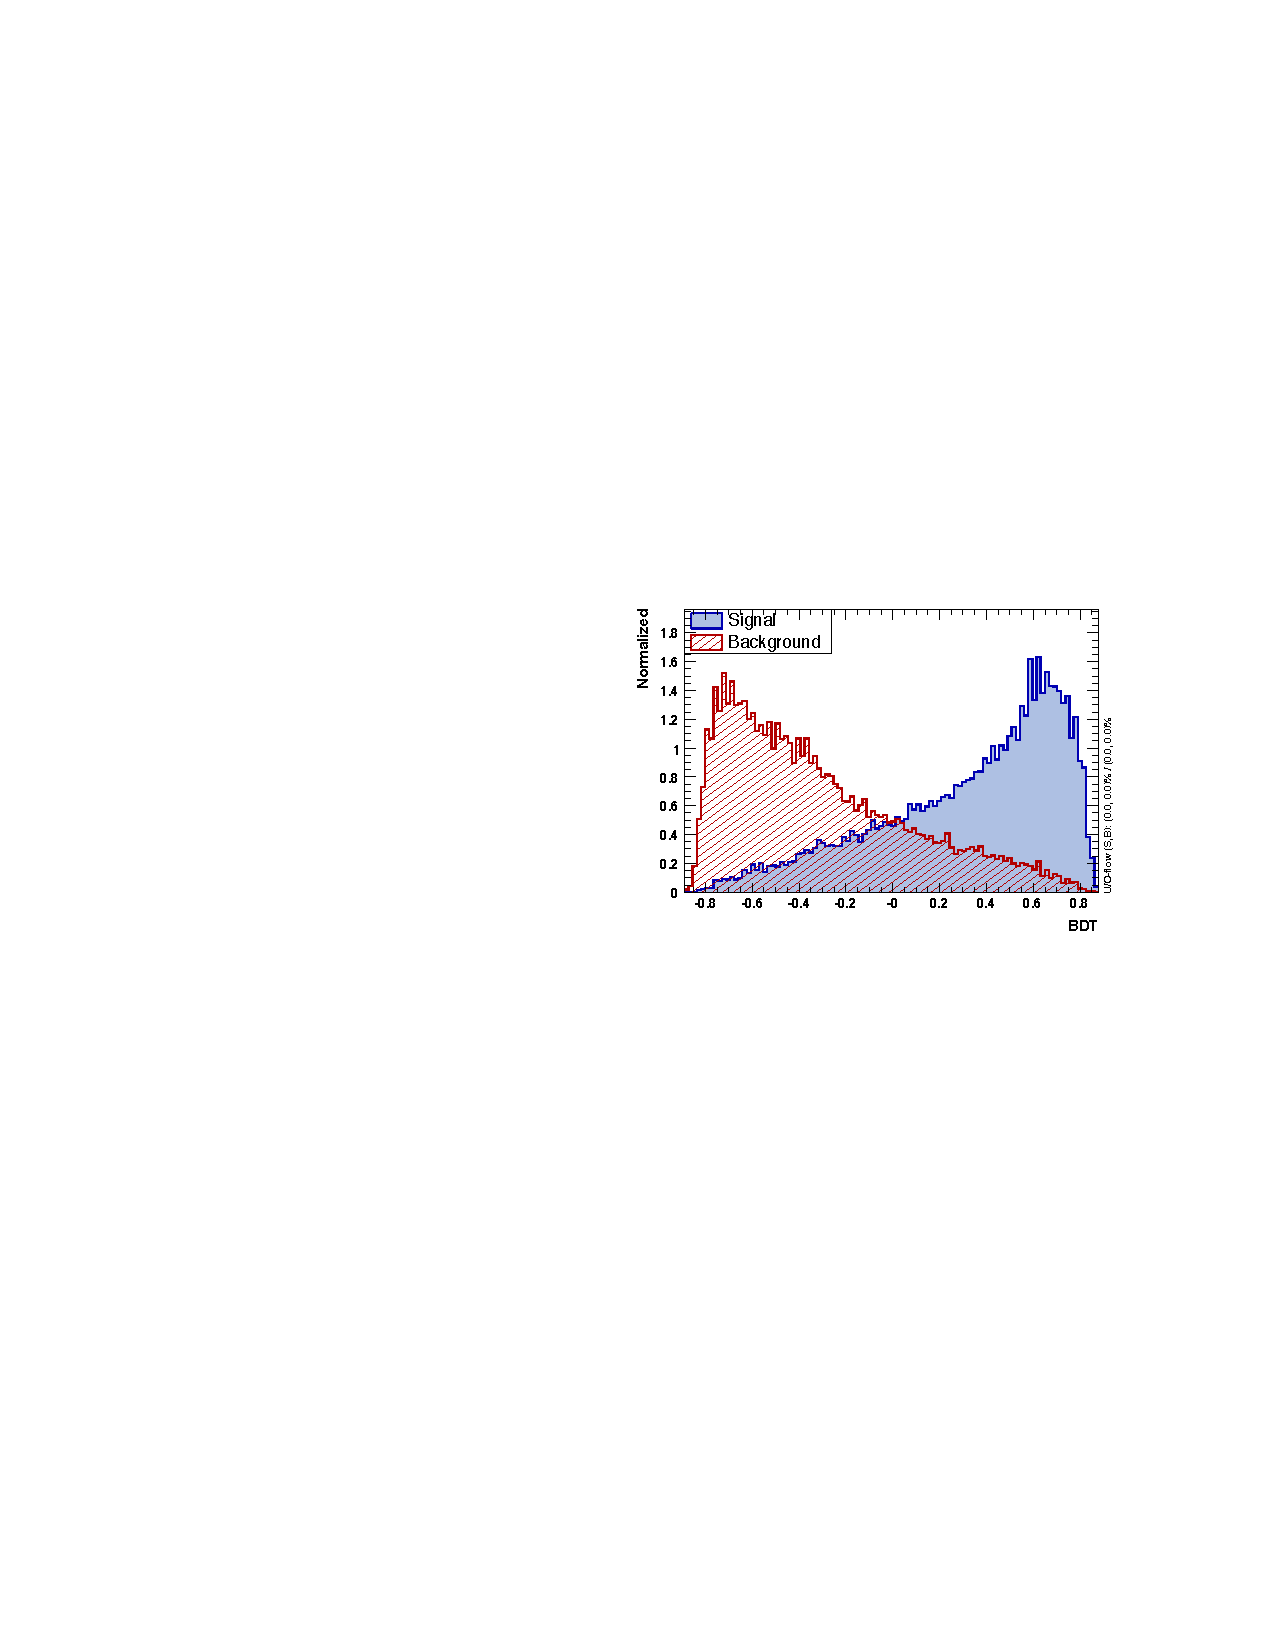
\includegraphics[height=1.7in]{figures/example-TMVA-BDT.pdf}
 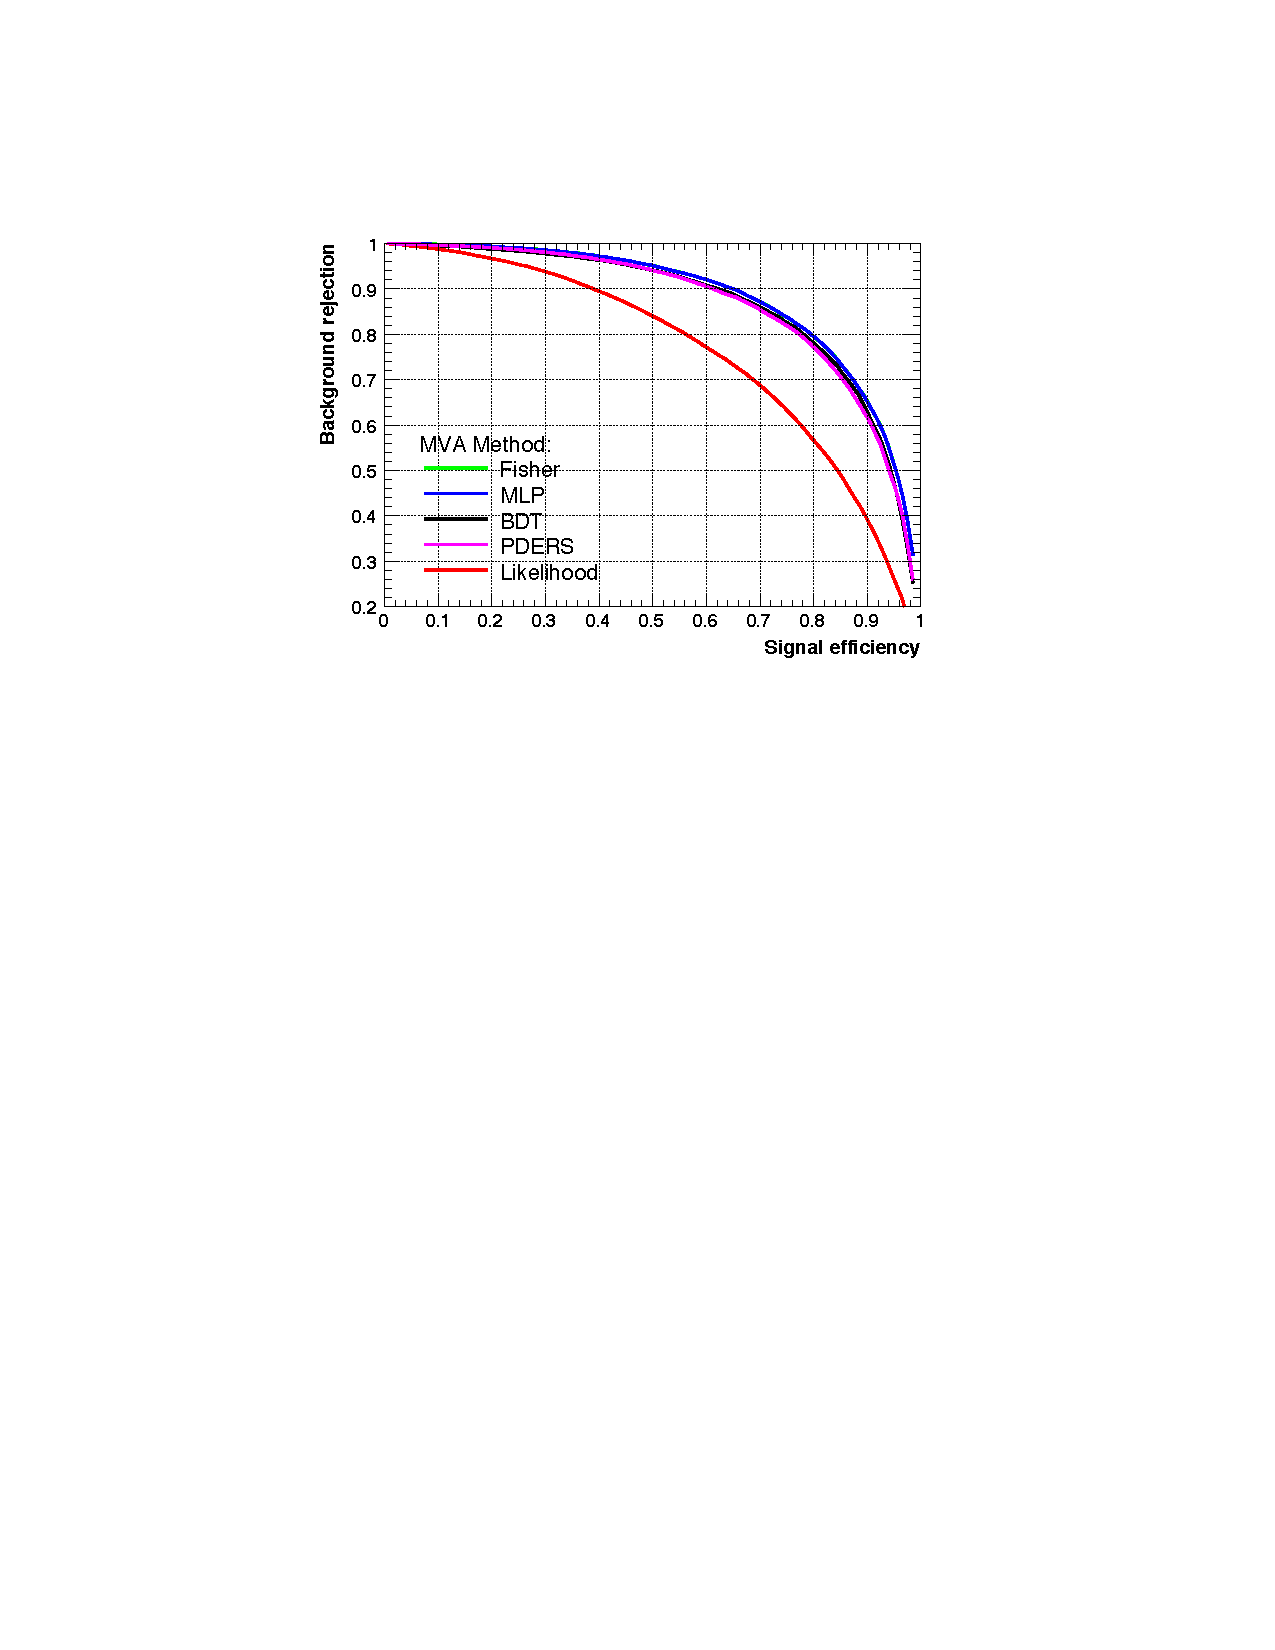
\includegraphics[height=1.7in]{figures/example-TMVA-ROC.pdf}
\caption{Left: an example of the distributions $p_b(\hat s|\nu)$ and $p_s(\hat s|\nu)$ when the classifier $s$ is a boosted-decision tree (BDT). Right: the corresponding ROC curve (right) for this and other classifiers. (Figures taken from TMVA manual.)}
\label{fig:tmva}
\end{center}
\end{figure}
%\bigskip

These steps feed into a subsequent statistical test based on the observed data
${D=(x_1, \dots, x_n)}$. For each event, the classifier is evaluated and one performs inference on a parameter $\mu$ related to the presence of the signal contribution. In particular, one forms the statistical model\footnote{Sometimes there is an additional Poisson term when expected number of signal and background events is known, which is referred to as an extended likelihood or marked Poisson model.}
\begin{equation}\label{eq:typicalML}
p( D \,|\, \mu, \nu) = \prod_{e=1}^n \, \left[\, \mu \hat{p}_s( \hat s(x_e) \, |\,  \nu)  + (1-\mu)\, \hat{p}_b( \hat s(x_e) \,|\, \nu) \,\right] \; .
\end{equation}

\subsection{Comments on typical usage of machine learning in HEP}

Nuisance parameters are an after thought in the typical usage of machine learning in HEP. In fact, most discussions would related to the training and optimizing the classifier only consider $p_b(x)$ and $p_s(x)$ with $\nu=\nu_0$ being implicit. However, as experimentalists we know that we must account for various forms of systematic uncertainty, parametrized by nuisance parameters $\nu$. In practice, we take the classifier as fixed and then propagate uncertainty through the classifier as in Eq.~\ref{eq:typicalML}. Building the distribution $p(\hat s|\nu)$ for values of $\nu$ other than the nominal $\nu_0$ used to train the classifier can be thought of as a calibration necessary for classical statistical inference; however, this classifier is clearly not optimal for $\nu \ne \nu_0$.

\subsection{A more powerful  approach}

The standard use of machine learning in HEP can be improved by training a parametrized classifier corresponding to the generalized likelihood ratio test
\begin{equation}
\lambda(\mu) = \frac{p(D|\mu, \hat{\hat{\nu}})}{p(D|\hat \mu, {\hat{\nu}})} \;,
\end{equation}
following the approach outlined in Section~\ref{S:GLR}.

There is an interesting distinction between this approach and the standard use in which the classifier is trained for a fixed $\nu_0$. In the standard use one trains a classifier for signal vs. background, which is equivalent (in an ideal setting) to training a classifier for  null (background-only) vs. alternate (signal-plus-backgound) since the resulting regression functions are one-to-one with each other.
In contrast, in the case of the generalized likelihood ratio test
\begin{equation}\label{eq:hep_improved}
 \frac{p(x| 0, \hat{\hat{ \nu}})}{p(x|\hat \mu, \hat\nu)} =  \frac{p_b(x| \hat{\hat{ \nu}})}{ \hat \mu p_s( x_e \, |\,  \hat\nu)  + (1- \hat \mu )\, p_b( x_e \,|\, \hat \nu)} \; ,
\end{equation}
the background components don't cancel and there is an additional term $p_b(x| \hat{\hat{ \nu}})/p_b(x| {\hat{ \nu}})$.
In practice, with classifiers of finite capacity, there will be some tradeoff between taking into account this additional term and the more challenging learning problem when $\mu$ is very small.

\subsection{Decomposing tests between mixture models into their components}

In this section we generalize the capacity focusing technique of training classifiers to discriminate between components of a mixture model. First, we generalize Eq.~\ref{eq:hepGen} to a mixture model of several components
\begin{equation}
p(x|\theta)=\sum_c w_c(\theta) p_c(x| \theta) \;.
\end{equation}
It is possible to re-write the target likelihood ratio between two mixture models in terms of pairwise classification problems.
\begin{eqnarray}\label{eq:decompose}
\frac{p(x|\theta_0)}{p(x|\theta_1)} & =& \frac{\sum_c w_c(\theta_0) p_c(x| \theta_0)}{\sum_{c'} w_{c'}(\theta_1) p_{c'}(x| \theta_1)}
\\
%&=& \sum_c \frac{ w_c(\theta_0) p_c(x| \theta_0)}{\sum_{c'} w_{c'}(\theta_1) p_{c'}(x| \theta_1)} \\
%&=& \sum_c \left[ \frac{\sum_{c'} w_{c'}(\theta_1) p_{c'}(x| \theta_1)}{ w_c(\theta_0) p_c(x| \theta_0)}  \right]^{-1} \\
&=& \sum_c \left[ \sum_{c'} \frac{ w_{c'}(\theta_1)}{w_c(\theta_0)} \frac{ p_{c'}(x| \theta_1)}{  p_c(x| \theta_0)}  \right]^{-1} \\ \label{eq:decomposedResult}
&=& \sum_c \left[ \sum_{c'} \frac{ w_{c'}(\theta_1)}{w_c(\theta_0)} \frac{ p_{c'}(s_{c,c',\theta_0, \theta_1}| \theta_1)}{ p_c(s_{c,c',\theta_0, \theta_1}| \theta_0)}  \right]^{-1}
\end{eqnarray}
The second line is a trivial, but useful decomposition into pair-wise classification between $p_{c'}(x|\theta_1)$ and $p_c(x|\theta_0)$.  The third line uses Theorem~1 to relate the high-dimensional likelihood ratio into an equivalent calibrated likelihood ratio based on the univariate density of the corresponding classifier, denoted $s_{c,c',\theta_0, \theta_1}$. In the situation where the only free parameters of the  model are the mixture coefficients $w_c$, then the distributions $p_{c}(s_{c,c',\theta_0, \theta_1}| \theta)$ are independent of $\theta$ and can be pre-computed (after training the discriminative classifier, but before evaluating the  likelihood ratio). Equation~\ref{eq:decomposedResult} allows one to take advantage of both the parametrized classifier as in Eq.~\ref{eq:hep_improved} and the capacity focusing technique in the typical HEP usage pattern.



\subsection{Measuring particle properties}

While the original motivation for this work was to improve the treatment of systematic uncertainties in new particle searches by parametrizing the classifier in terms of the nuisance parameters $\nu$, the same approach can be used for parameter inference. In the case of new particle searches the parameter of interest is the mixture coefficient for the signal component $p_s(x|\nu)$. When measuring particle properties the distribution of the features also depend on parameters such as a particle's mass and quantum numbers. This is easily accommodated by extending $p_s(x|\nu) \to p_s(x|\theta)$, where $\theta$ includes both parameters of interest and nuisance parameters.

This formalism represents a significant step forward in the usage of machine learning in HEP, where classifiers have always been used between two static classes of events and not parametrized explicitly in terms of the physical quantities we wish to measure. The work of  ~\citep{Whiteson:2006ws} is similar as the stochastic optimization was directly trying to minimize the measurement uncertainty of a particle's mass; however, the resulting classifier was fixed. This approach also offers the advantage that it explicitly reformulates the per-experiment optimization to the per-event optimization, which is less computationally intensive.

Another approach that is similar in spirit is the so-called matrix element method, in which one  directly computes an approximate likelihood ratio by performing a computationally intensive integral associated to the detector response~\citep{Volobouev:2011vb}. In the approach considered in this paper, the detector response is naturally handled by the Monte Carlo sampling used in the simulation of the detector; however, that integral is intractable for the matrix element method. Even with drastic simplifications of the detector response, the matrix element method can take several minutes of CPU time to calculate the likelihood ratio $q(x)$ for a single event. The work here can be seen as aiming at the same conceptual target, but utilizing machine learning to overcome the complexity of the detector simulation. It also offers enormous speed increase for evaluating the likelihood at the cost of an initial training stage. In practice, the matrix element method has only been used for searches and measurement of a single physical parameter (sometimes with a single nuisance parameter as in~\citep{Aaltonen:2010yz}).

Contemporary examples where the technique presented here could have major impact on HEP include the measurement of coefficients to quantum mechanical operators describing the decay of the Higgs boson~\citep{Chen:2014pia} and, if we are so lucky, measurement of the mass of supersymmetric particles in cascade decays~\citep{Allanach:2000kt}.  Both of these examples involve data sets with many events, each with a feature vector $x$ that has on the order of 10 components, and a parameter vector $\theta$ with 5-10 parameters of interest and possibly many more nuisance parameters.
The state of the art for the operator coefficients of the Higgs decay uses the so-called matrix element likelihood analysis (MELA) in which the equivalent of $s(x; \theta_0, \theta_1)$ is approximated by neglecting detector effects~\citep{Gao:2010qx,Bolognesi:2012mm}.

\bigskip

\section{Related work}\label{S:Related}


\citep{ClaytonScott} and \citep{JMLR:v14:tong13a} consider the machine learning problem associated to Neyman-Pearson hypothesis testing. As in this work, they consider the situation where one does not have access to the underlying distributions, but only has i.i.d. samples from each hypothesis. This work generalizes that goal from the Neyman-Pearson setting to generalized likelihood ratio tests and emphasizes the connection with classification. Perhaps a  formal treatment similar to the Neyman-Pearson case can be brought to bear in this more general setting.
In a similarly titled work, \citep{Gutmann2014} advocate using the cross-validated classification accuracy as the similarity metric used in ABC. While the goal there is also parameter inference in the likelihood-free setting,  ``classifier ABC'' is very different than the approach presented here.
\citep{TommiJaakkola} explore a way of leveraging generative models to derive kernel functions for use in discriminative methods. This interesting work is distinct from the point made here in which the generative model is being used for the purpose of providing training data and calibration.
%\citep{McCallum} consider a hybrid generative/discriminative classifier; however, the goal of that work is not to leverage a generative model for the data, but to use both approaches to learn different subsets of the parameters in a single hybrid classifier.
\citep{BiancaZadrozny} emphasize the importance of calibrated probability estimates from decision trees and naive Bayesian classifiers and investigate various approaches to achieve this. In contrast to that work, we are not interested in calibrated probability estimates for $p(y|x)$ for individual events, but instead we use the calibration to correct for non-linear transformations of the target likelihood ratio and, perhaps, to provide calibrated p-values based on those likelihood ratio tests. \citep{Ihler2004} take on a different problem (tests of statistical independence) by using machine learning algorithms to find  scalar maps from the high-dimensional feature space that achieve the desired statistical goal when the fundamental high-dimensional test is intractable.


\citep{Neal:2007zz} also considered the problem of approximating the likelihood function when only a generative model is available. That work sketches a scheme in which one uses a classifier with both $x$ and $\theta$ as an input to serve as a dimensionality reduction map.
The key distinction comes in the handling of $\theta$.  Neal says  ``we cannot use the classifier on real data, since we don't know the correct value for [$\theta]$'' and goes on to outline an approach where one uses regression on a per-event basis to estimate $\hat{\theta}(x)$ and perform the composition $s(x; \hat{\theta}(x))$ (much like profiling).\footnote{Neal considers a lower-dimensional `bottlenecks' $\theta^*=g(\theta)$, which are not essential to the discussion here.}  This can lead to a significant loss of information since (at least in most particle physics examples) a single event carries little information about the true value of $\theta$, though the full data set $D$ may be informative -- for instance, a single observation would not be sufficient to estimate the variance of a distribution, though repeated observations would.  The work of Neal correctly identifies this as an approximation of the target likelihood even in the case of a ideal classifier. In contrast, the approach described here does not eliminate the dependence of the classifier on $\theta$.%
\footnote{As a technical point, in Neal's work, the focus is on approximating the likelihood function (up to a multiplicative constant), which is equivalent to evaluating the ratio  with respect to a fixed $\theta_1$ as in Eq.~\ref{eq:mle_withs}. In Neal's case, the dependence on $\theta$ is eliminated via $s(x; \hat{\theta}(x))$ and the map is constant; however, in this approach the map ratio is explicitly parametrized in terms of $\theta$, so the ratio is important for canceling the corresponding Jacobian factors.} Instead, we embed a parametrized classifier into the likelihood and postpone the evaluation of the classifier to the point of evaluation of the likelihood when $\theta$ is explicitly being tested. This avoids the loss of information that occurs from the regression step $\hat{\theta}(x)$ proposed by Neal and leads to Theorem~1, which is an exact result in the case of an ideal classifier. In both cases, the quality of the classifier is factorized from the calibration of its density, which allows for valid inference even if there is a loss of power due to a non ideal classifier.



\section{Conclusions}

We have outlined a technique to reformulate generalized likelihood ratio test over a high-dimensional data set with multiple events in terms of a univariate density of a classifier score.
We have shown that a parametrized family of discriminative classifiers $\hat s(x; \theta_0, \theta_1)$ trained and calibrated with a simulator  $p(x|\theta)$ can be used to approximate the  likelihood ratio  $\prod_i p(x_i|\theta_0)/p(x_i|\theta_1)$ even when it is not possible to directly evaluate the likelihood $p(x|\theta)$.
%A technique for decomposing this ratio when the generative model is a mixture of components was presented with the aim to help focus capacity of the classifier when $p(x|\theta_0)$ and $p(x|\theta_1)$ differ primarily by a small mixture coefficient.  This approach leverages the power of machine learning in a classical statistical setting.
It offers an alternative to approximate Bayesian computation for parameter inference in the likelihood-free setting that can also be used in the frequentist formalism without specifying a prior over the parameters. A strength of this approach is that it separates the quality of the approximation of the target likelihood from the quality of the calibration. The former is related to the ability of supervised learning approaches to  classification, which will continue to improve. The calibration procedure for a particular parameter point is fairly straight forward since it involves estimating a univariate density using a generative model of the data. The difficulty of the calibration stage is performing this calibration continuously in $\theta$. Different strategies to this calibration are anticipated depending on the dimensionality of $\theta$, the complexity of the resulting likelihood function, and the difficulties associated to running the simulator.








\bibliographystyle{apalike}
\bibliography{learning.bib}

\end{document}
